\documentclass{elegantpaper}

\usepackage{algorithm}
\usepackage{algorithmicx}
\usepackage{algpseudocode}

\floatname{algorithm}{算法}
\renewcommand{\algorithmicrequire}{\textbf{输入:}}
\renewcommand{\algorithmicensure}{\textbf{输出:}}

\title{分布式空间top-k频繁关键字查询}

\begin{document}

\maketitle

\begin{table}[!htbp]
    \centering
    \begin{tabular}{ccc}
    姓名&学号&分数占比\\
    \hline
    冯运&1160300524&50\%\\
    陈进龙&1160300525&50\%\\
    \end{tabular}
\end{table}

\begin{abstract}
    top-K频繁项查询一直是一个热门的研究方向,而随着互联网的社交的快速发展,空间top-k频繁项查询问题也有了很广泛的应用场景,并且由于数据量的爆炸性增长,单机运行的查询系统已经不能满足实际生产的需要。在这篇论文中,我们把问题定义为用户制定一个查询的空间和需要的项数k,由系统返回在这个空间中出现的最频繁的k个数据项,并且从原始数据的导入,存储,到查询检索等过程全部实现分布式计算.为了解决这个问题,我们使用了一种分布式的多维数据索引结构MC-R树来存储和索引数据,这种结构适用于任意的数据规模.我们还针对此结构存在的性能问题进行结构性优化,使得整个系统可以同时应对大量的查询请求,快速而准确的返回计算结果,并且具有良好的横向扩展性,能够灵活应对不同查询规模,不同的查询次数.
\end{abstract}

\section{问题描述}

随着社交软件的大量出现,许多社交平台允许用户在发布消息的时候会标记他们的地理位置,例如微博,微信朋友圈等.这样的背景条件下,就产生了新的数据分析问题.例如,当用户想去知道附近的热门地点时,需要对已经产生的地点信息进行计算,即用户给定一片空间区域,然后查询返回k个最热门的关键词,而随着数据产生的越来越多,数据量的存储已经远远超过了一个单机的能力,所以分布式的空间top-k关键字查询就成为了新的数据分析需求.

\subsection{形式化描述}
我们使用$L=\{o_1,o_2,o_3,...,o_n\} $ 来表示一个包含N个o对象的数据集,每一个对象$o_i$是<Place,Words>形式的对象.Place是一个n维的的空间坐标点,用$Place=\{w_1,w_2,...\}$来表示,而Words是对象o保存的关键字,用$Words=\{w_1,w_2,w_3... \}$.\newline
使用$V=\{U_{o\in L}O.Words\}$来表示L内的所有关键词的集合,使用$f_o(w)$来表示关键词$w$出现在对象o中的次数.\newline
对于一个给定的查询区域R,则可以用$f_R(w)=\{\sum{f_{oi(w)|o_i.Place\in R}} \}$来表示关键词w在区域R中出现的频率(次数).\newline
对于这个top-k频繁关键词查询系统来说,输入一个查询条件:$<R_Q,k>$,$R_Q$指明了选择的查询区域,k指明了最终输出的k个关键字,而这k个关键字是出现在$R_Q$区域内的k个最高频的关键字.\newline

\subsection{举例}

例如figure1表示的是一个二维的平面,其中包含了8个对象,则可以用$L=\{o_1,o_2,o_3,o_4,o_5,o_6,o_7,o_8\}$,每一个对象对应的关键词组在table1中展示
假设用户的查询是$Query=<R_4,3>$,即查询的区域是R4,用户要求的k=3的情况下,需要返回在区域R4中的top-3频繁的关键字,而从figure1中可以看出,在R4中包含的对象有$\{o_4,o_6,o_7,o_8\}$,根据table1可以算出最终的top-3为$\{w_2,w_3,w_9\}$.

\begin{figure}[!ht]
	\centering
	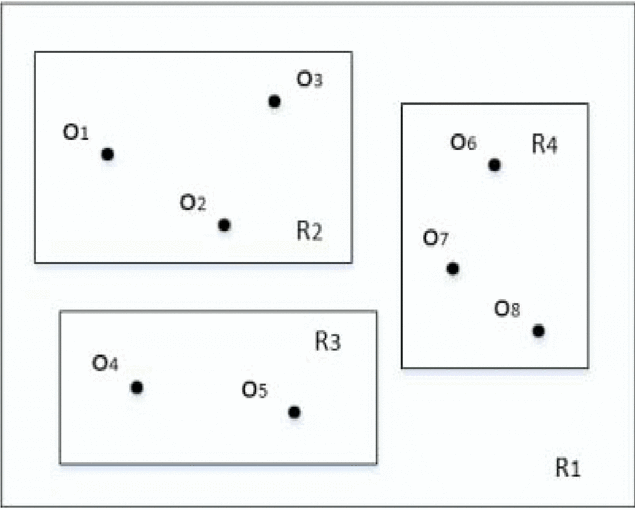
\includegraphics[width=0.6\textwidth]{figure1.png}
	\caption{空间示意图\label{fig:figure1}}
\end{figure}

\begin{table}[!htbp]
    \centering
    \caption{对象的关键词}
      \begin{tabular}{cccc}
      对象&关键词&对象&关键词\\
      \hline
      $o_1$   & $\{w_2,w_3,w_5\}$ & $o_5$&$\{w_1,w_1,w_3,w_5\}$\\
      $o_2$   & $\{w_1,w_4,w_5\}$ & $o_6$&$\{w_4,w_7,w_9\}$\\
      $o_3$   & $\{w_2,w_4,w_4\}$ & $o_7$&$\{w_2,w_2,w_3,w_5\}$\\
      $o_4$   & $\{w_3,w_8,w_9,w_9\}$ & $o_8$&$\{w_3,w_3,w_6\}$\\
      \end{tabular}
\end{table}

\section{系统设计}

本节首先介绍一种分布式的索引结构,并基于此结构实现一种简单的查询算法。然后介绍基于此设计的一些改进以及相应的新的查询算法。

\subsection{索引结构}

对于空间数据索引,首选的结构就是R树。
但是传统的R树是基于单机的,没有考虑分布式计算的需求,这里我们介绍一种分布式的R树 [1] ,可以满足并行计算的要求。

\subsubsection{MC-R树}

MC-R树是一种分布式的多维数据索引结构,它将物理计算节点分为两类:

\begin{itemize}

    \item Master节点:保存全局索引信息。Master维护着一个\verb|<MBR, client_id>|的列表以及在其上的R树索引,用于将查询转发到相应的Client节点;
    
    \item Client节点:负责保存局部索引以及数据。Client节点保存实际的数据分块以及在这些数据上建立的局部R树索引;
    
\end{itemize}

\begin{figure}[!ht]
    \centering
    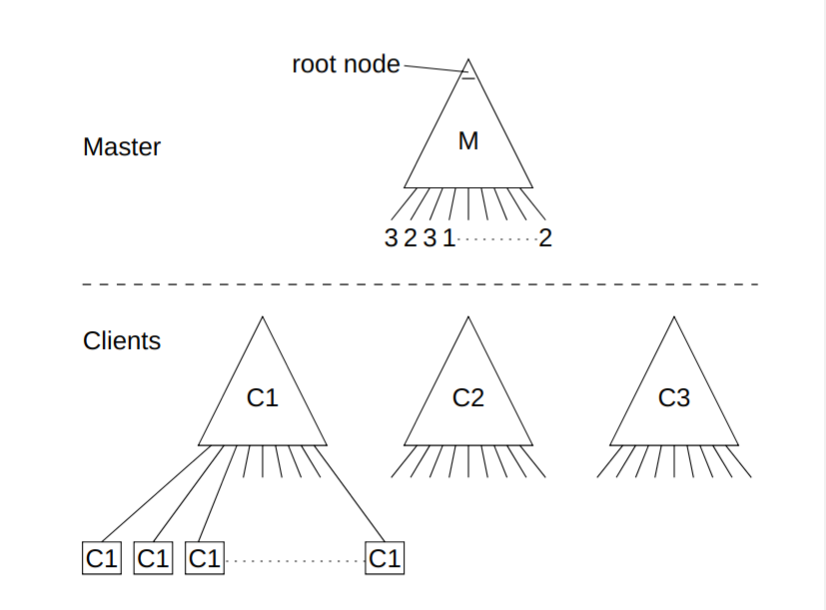
\includegraphics[width=0.6\textwidth]{figure/MC-Rtree.png}
    \caption{MC-R树的结构,其中三角形表示物理节点,四边形表示数据}
\end{figure}

\subsubsection{MC-R树的建立过程}

\begin{itemize}
    
    \item[1.] 数据划分:Master节点将导入的按照特定的划分算法数据划分为G组,每一组最多M个数据。其中M是每一个物理节点能保存的最大数据量;
    
    \item[2.] 数据分配:数据划分完成后,将每一组数据分配给一个Client节点,并将该次分配产生的\verb|<MBR, client_id>|二元组添加到列表中;
  
    \item[3.] 建立全局索引:Master将数据分配到Client节点后,在分配过程中产生的\verb|<MBR, client_id>|列表上建立R树索引;
    
    \item[4.] 建立局部索引:收到数据的Client节点将数据保存到本地磁盘,然后在这些数据上建立局部R树索引。
 
\end{itemize}

\subsubsection{两种典型的多维数据划分算法}

\begin{itemize}
    
    \item Hilbert packing算法:将所有的数据(超立方体)按照它们的中心到希尔伯特曲线起点的距离进行排序,然后将排序结果等距离的划分为G段即可。

    \item Sort-Tile-Recursive(STR)算法:对于n个k维的数据(超立方体),首先确定需要划分成的份数$G = \lceil \frac{n}{M} \rceil$。接下来将这些超立方体按照它们中心的第一维坐标进行排序,将排序结果等距离地分为$S = \lceil G^{\frac{1}{k}} \rceil$份,然后递归的对每一份的$k - 1$维坐标进行处理,最终得到划分结果。

\end{itemize}

\subsubsection{MC-R树的查询}

对MC-R树的查询都会被发送到Master节点,Master节点找出选择与查询区域相交的Client节点并将查询发送给它们。
每一个Client节点收到查询后即在本地执行查询,并将查询结果返回给Master,Master负责汇总所有查询结果并返回给用户。

\noindent 针对空间top-k频繁关键字问题,具体的查询算法如下:

\begin{itemize}
    
    \item[1.] 在MC-R树叶节点保存的数据包括本节点的MBR以及由形似\verb|<t, entries, freq>|的三元组组成的列表,其含义为:
              
              \begin{itemize}
                  
                \item {\bfseries t:} 在本区域出现的关键字;
                
                \item {\bfseries entries:} 形似\verb|<loc, freq>|的二元组组成的列表,表示关键字\verb|t|出现的所有位置及在该位置出现的次数;
                
                \item {\bfseries freq:} 该关键字在本区域出现的总次数;

              \end{itemize}

    \item[2.] 查询首先发送给Master,Master再将查询发送给相关的Client,同时记录下查询被发给了哪些Client;
    
    \item[3.] 每个Client收到查询后,找到出本区域内与查询区域相交的所有叶节点,对于每个叶节点,按照以下算法求出其中的位于查询区域内的关键字及其出现次数并返回给Master:\\\\\\\\\\\\\\\\\\\\
    
              \begin{algorithm}

                \begin{algorithmic}[1]
                    \caption{MC-R树叶节点查询算法}
                    \Require 叶节点$R$, 查询$Q$
                    \Ensure $R$中位于查询区域$Q.MBR$内的关键字及其出现次数

                    \Function {Query}{$R, Q$}
                        \State $KWFreq = \{\}$
                        \If {$R.MBR \subseteq Q.MBR$}
                            \For {$entry$ in $R.entries$}
                                $KWFreq = KWFreq \bigcup \{<entry.t, entry.freq>\}$
                            \EndFor
                        \Else
                            \For {$entry$ in $R.entries$}
                                \State $FreqSum = 0$
                                \For {$tentry$ in $entry.entries$}
                                    \If {$tentry.loc \in R.MBR$}
                                        \State $FreqSum = FreqSum + tentry.freq$
                                    \EndIf
                                \EndFor
                                \If {$FreqSum > 0$}
                                    $KWFreq = KWFreq \bigcup \{<entry.t, FreqSum>\}$
                                \EndIf
                            \EndFor
                        \EndIf
                        \State \Return {$KWFreq$}
                    \EndFunction
                    
                \end{algorithmic}
                  
              \end{algorithm}
    
    \item[4.] Master收到所有与当前查询相关的Client返回的\verb|<t, freq>|二元组列表后,对这些列表进行合并,统计出每一个关键字出现的总次数,进而找出出现次数最多的k个关键字并返回给用户。

\end{itemize}

\subsection{查询优化}

分析以上基于MC-R树的查询过程可以发现,直接将Client的查询结果返回给Master汇总的处理方式存在以下两个比较明显的问题:

\begin{itemize}

    \item Master负载过重:由于所有查询结果都需要交给Master进行汇总,当查询数量过多时Master将成为整个系统的性能瓶颈;
    
    \item 对于每个查询,Master需要维护查询到的所有关键字的出现次数,当关键字过多时,这将占据大量的资源,然而事实上用户可能只需要其中很小的一部分;
    
\end{itemize}

\noindent 针对以上两个问题,我们引入了一些新的物理节点,减轻了Master的负载,并且避免了维护过多查询结果造成的资源浪费。

\subsubsection{查询分配节点QueryMaster}

QueryMaster是代替原来的Master直接与用户交互的节点。QueryMaster维护着所有的QueryManager以及它们的负载情况(正在处理的请求数),当一个查询请求到来时,QueryMaster为该请求分配一个id,并根据各个QueryManager的负载情况将请求分配给负载最轻的QueryManager。

\subsubsection{查询管理集群QueryManagers}

QueryManagers是一组用于管理用户查询的计算节点,每一个QueryManger负责维护一些查询请求,一个查询请求包括:

\begin{itemize}

    \item 查询id:由QueryMaster分配,用于标识一个查询请求;
    
    \item 查询$<R_Q, k>$:用户提交的查询;
    
    \item 一个容量为$k$的小根堆MinHeap:用于统计出top-k;
    
    \item 负责该次查询的Client列表;
    
    \item 负责该次查询的Aggregator列表;
    
\end{itemize}

\subsubsection{聚集集群Aggregators}

Aggregators是一组专门负责聚集Client查询结果的计算节点。每一个Aggregator负责一些关键字的聚集,它从Client处接收\verb|<t, freq>|键值对,然后对所有Client发给它的键值对进行聚集,并将聚集结果的top-k发送给相应的QueryManager。

\noindent 每个Aggregator维护着一系列形如\verb|<query_id, entries>|的键值对,其键为查询id,值为一系列形如\verb|<t, freq>|的键值对,表示在该查询中关键字t出现的次数。Client按照相同的格式发送查询结果给Aggregator,Aggregator按照如下算法进行聚集:\\\\\\\\\\\\\\\\\\\\\\\\

\begin{algorithm}

    \begin{algorithmic}[1]
        \caption{Aggregator聚集算法}
        \Require Aggregator $A$, Client发来的键值对$<query\_id, entries>$

        \Function {aggregate}{$A, <query\_id, entries>$}
            \If {$query\_id \in A.keys()$}
                \State $originalEntries = A.get(query\_id)$
                \For {$<t, freq>$ in $entries$}
                    \If {$t \in originalEntries.keys()$}
                        \State {$newFreq = freq + originalEntries.get(t)$}
                        \State {$originalEntries.put(t, newFreq)$}
                    \Else
                        \State {$originalEntries.put(t, freq)$}
                    \EndIf
                \EndFor
            \Else
                \State {$A.put(query\_id, entries)$}
            \EndIf
        \EndFunction
        
    \end{algorithmic}
    
\end{algorithm}

\subsection{最终结构}

经过优化以后,我们将整个系统分为三个部分:

\begin{itemize}

    \item Query Group:包含一个QueryMaster和一组QueryManager,QueryMaster负责维护所有的QueryManager以及它们的负载情况,为查询指定id以及将查询分配到QueryManager;QueryManager负责维护查询的状态以及执行查询结果的最终汇总;

    \item Index Group:包含一个IndexMaster和一组Client,IndexMaster是作为全局索引,负责返回与给定查询相关的所有Client;Client作为数据节点,需要在本地数据上建立局部索引,负责执行查询并将查询结果发送给Aggregator Group做聚集;
    
    \item Aggregator Group:包含一组Aggregator,每一个Aggregator负责一些关键字的聚集;
    
\end{itemize}

\noindent 各个部分之间的关系如下:\\\\\\\\

\begin{figure}[htbp]
    \centering
    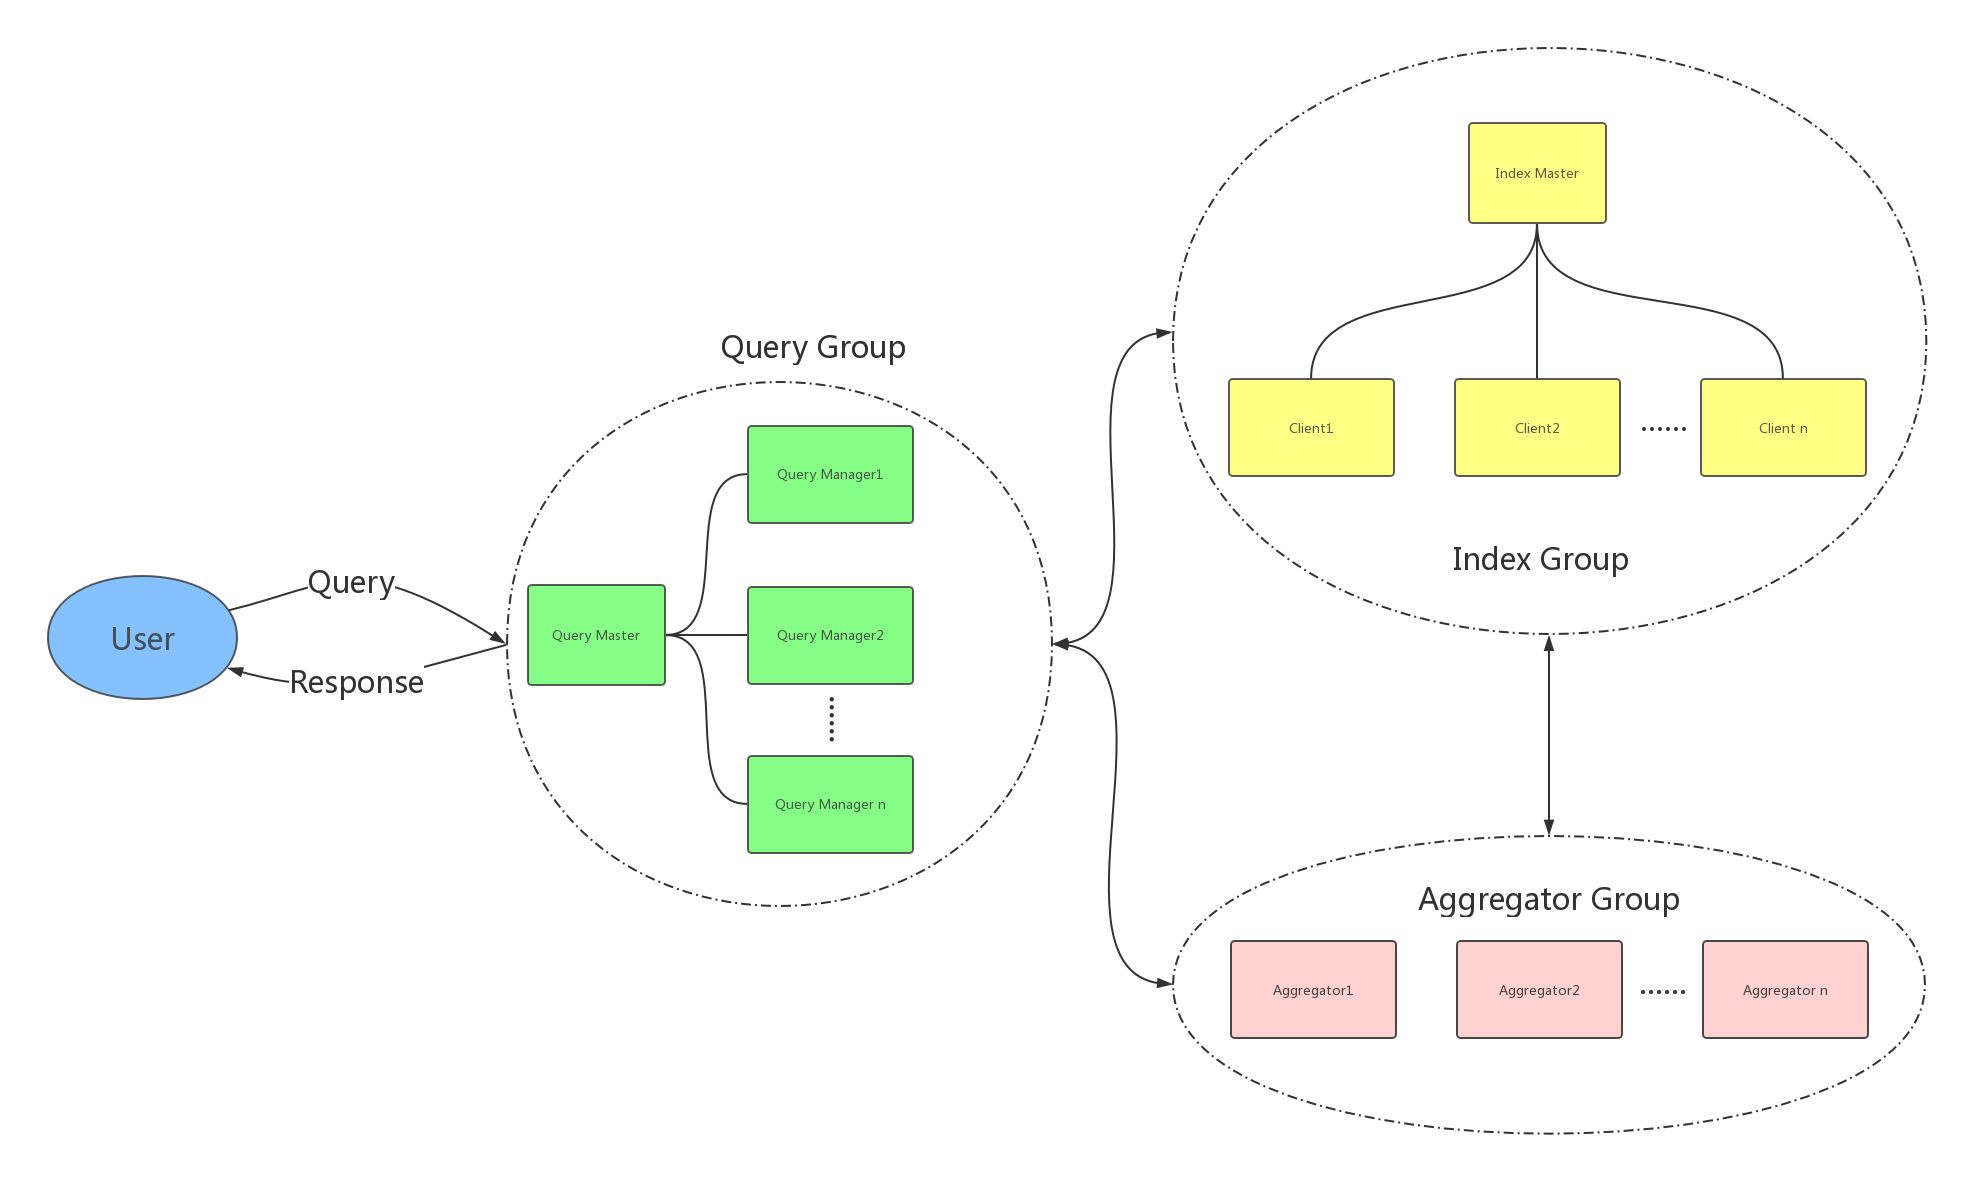
\includegraphics[width=1\textwidth]{figure/architecture.png}
    \caption{系统架构图}
\end{figure}

\section{工作流程}
\subsection{查询集群QueryGroup}
\begin{itemize}
    \item[1.] 用户向查询集群QueryGroup的QueryMaster结点发送查询请求$q_i=<R_Q,k>$,QueryMaster为这个请求编号为$q_i$;
    \item[2.] QueryMaster根据QueryGroup中各QueryManager的负载情况,将查询$q_i$分配给某一QueryManager,假设为$QM_j$;
    \item[3.] $QM_j$收到这个查询请求后,为这个请求做相应的初始化工作,包括创建一个容量为$k$的小根堆MinHeap,创建一个ClientList(用于保存需要$QM_j$需要查询的IndexGroup中的Client结点),创建一个AggregatorList(用于保存在此次查询中用到的Aggregator结点);
    \item[4.] $QM_j$向MC-R树(IndexGroup)的IndexMaster结点发送请求$q_i$,IndexMaster返回查询得到的Client结点,$QM_j$将这些Client结点添加进QueryList中;
    \item[5.] $QM_j$向QueryList中的所有Client发送查询请求;
    \item[6.] $QM_j$等待已请求的Client结点返回确认信息,确认信息中包括了该Client节点需要的所有Aggregator结点。$QM_j$将这些Aggregator去重后添加到AggregatorList中;
    \item[7.] 当$QM_j$收到QueryList所有中的Client结点发来的确认信息后,向AggregatorList中的所有Aggregator结点请求查询$q_i$的聚集结果;
    \item[8.] 对于Aggregator发来的每一个聚集结果\verb|<query_id, entries>|,$QM_j$按照如下算法进行汇总:
              \begin{algorithm}

                \begin{algorithmic}[1]
                    \caption{QueryManager汇总算法}
                    \Require 一个聚集结果\verb|<query_id, entries>|

                    \Function {combine}{$<query\_id, entries>$}
                        \State $MinHeap = getMinHeapOf(query\_id)$
                        \For {$entry$ in $entries$}
                            \If {$!MinHeap.isFull()$}
                                \State $MinHeap.insert(entry)$
                            \Else
                                \If {$entry.freq > MinHeap.top().freq$}
                                    \State $MinHeap.pop()$
                                    \State $MinHeap.insert(entry)$
                                \EndIf
                            \EndIf
                        \EndFor
                    \EndFunction
                    
                \end{algorithmic}
                  
              \end{algorithm} 
    \item[9.] 如果$QM_j$收到了参与$q_i$查询的聚集任务的所有Aggregator发来的聚集结果,则MinHeap中的所有关键词就是最终需要的结果;
    \item[10.] $QM_j$将MinHeap中的所有结果进行汇总和封装,返回给用户;
    \item[11.] 释放此次查询所占用的全部资源,包括MinHeap,QueryList,AggregatorList等;
\end{itemize}
\subsection{索引集群IndexGroup}
\begin{itemize}
    \item[1.] 对应于查询集群(QueryGroup)中的步骤4,MC-R树(IndexGroup)中的IndexMaster结点收到结点$QM_j$的查询请求后,根据请求中的查询区域$R_Q$,检索自己的已有的全局索引,与查询区域相交的所有Client结点,将这些结点返回给结点$QM_j$;
    \item[2.] 对应于查询集群(QueryGroup)中的步骤5,MC-R树(IndexGroup)中的Client节点收到结点$QM_j$的查询请求后,按照以下算法执行查询并将查询结果发送给AggregatorGroup:
              \begin{itemize}

                \item[(1).] 通过局部索引找到所有与查询区域$R_Q$相交的叶节点,然后按照{\bfseries 算法1 MC-R树叶节点查询算法}求出本节点中所有位于查询区域内的关键字及其出现次数;
                
                \item[(2).] 对于每一个\verb|<t, freq>|键值对,计算关键字\verb|t|的哈希值,根据哈希值为该键值对选择一个Aggregator,记录下选择的Aggregator;
                
                \item[(3).] 将需要发送给同一Aggregator的所有键值对组合成一个列表\verb|entries|,然后将键值对\verb|<query_id, entries>|发送给相应的Aggregator;
                  
              \end{itemize}
    \item[3.] 对应于查询集群(QueryGroup)中的步骤6,Client结点向Aggregator发送完查询$q_i$的查询结果后,再将本次查询中用到的所有Aggregator去重后发送给$QM_j$,表明自己已经完成查询的分发;
\end{itemize}
\subsection{聚集集群AggregatorGroup}
\begin{itemize}
    \item[1.] 对应于索引集群(IndexGroup)中的步骤2,每个Aggregator按照{\bfseries 算法2 Aggregator聚集算法}对收到的查询结果进行聚集;
    \item[2.] 对应于查询集群(QueryGroup)中的步骤7,每个Aggregator在收到$QM_j$的请求后,将属于查询$q_i$的聚集结果中的top-k发送给$QM_j$,并清空属于查询$q_i$的所有聚集结果;
\end{itemize}
\end{document}